\documentclass[a4paper,12pt,oneside,English]{article}
\usepackage[a4paper,top=1.5cm,bottom=1.5cm,left=1cm,right=1cm]{geometry}
\usepackage[utf8]{inputenc}
\usepackage[T1]{fontenc}
\usepackage{blindtext}
\usepackage{framed}
\usepackage[svgnames]{xcolor}
\usepackage{graphicx}
\definecolor{shadecolor}{gray}{0.9}
\usepackage{mathtools}
\usepackage{caption}
\usepackage{subcaption}
\usepackage{dsfont}
\usepackage{nccmath}
\usepackage{graphicx}
\usepackage{amsthm}
\usepackage{color} 
\usepackage[pdftex,backref,linktocpage,colorlinks]{hyperref}
\usepackage{xcolor}
\usepackage{empheq}
\usepackage{adjustbox}
\usepackage{graphicx}
\usepackage{amssymb}
\usepackage{amsmath}
\usepackage{siunitx}
\usepackage{framed}
\usepackage{graphicx}
\documentclass[xcolor=table]{beamer}
\usepackage[table,xcdraw]{xcolor}
\usepackage[authoryear]{natbib}
\hypersetup{
    colorlinks,
    linkcolor={red!50!black},
    citecolor={red!50!black},
    urlcolor={red!50!black}
}
\usepackage{titling}
\usepackage{fancyhdr}
\usepackage[shortlabels]{enumitem}
\usepackage{float}
\usepackage[nottoc, notlof]{tocbibind}
\usepackage{setspace}
\usepackage[T1]{fontenc}
\usepackage{amsfonts}
\usepackage{amsmath}
\usepackage{indentfirst}
\renewcommand{\baselinestretch}{1.5}
\setlength{\skip\footins}{5ex plus 4pt minus 2pt}
\usepackage{rotating}
\usepackage{tocloft}
\setlength{\cftaftertoctitleskip}{1cm}
\setlength{\cftafterloftitleskip}{1cm}
\usepackage{enumitem}
\usepackage{titletoc,tocloft}
\setlength{\cftsubsecindent}{0cm}
\usepackage{floatflt} 
 \usepackage[bf, small]{caption}
 \usepackage[justification=centering]{caption}
 \setcounter{secnumdepth}{0}
\title{Problem set 1 - Sem 2}
\author{ Giacomo Lo Conte, Kun Wu, Francesca Eustacchi and Neeharika Kakunuri }

\begin{document}
\maketitle
\section{ 1 Theory I: DAGs and Potential Outcomes}
\textbf{a) Consider the following threshold model with a binary treatment $D$, an additional (binary) covariate} $x$\textbf{, the outcome} $y$ \textbf{and an i.i.d error term with mean zero} $\epsilon_i$
\begin{equation}
    y_i = \alpha + \beta D_i + \gamma x_i + \rho \epsilon_i
\end{equation}
\begin{equation}
\label{eqn 2}
 x_i = \mathds{1}(\kappa + \delta D_i + \pi \epsilon_i > c) 
\end{equation}

\textbf{The second part of equation \ref{eqn 2} means that} $x_i = 1$ \textbf{if the sum on the right hand side is greater than a threshold c and $x_i = 0$ otherwise. Assuming that} $\delta = 0$\textbf{, show that the estimator of the average treatment effect (ATE), }$\Delta=E(y|D = 1 ,x = X) - E(y|D = 0 ,x = X)$ \textbf{equals}  $\beta$ + \textit{bias}\textbf{, characterise the bias (i.e. derive the exact formula)  and explain what the bias means.}\\

Consider the expected value of $y$ conditioned to $x=X$ and $D=0$ or $D=1$. 
\begin{equation}
\begin{split}
        y_{D=1}&=E[y|D=1, x=X]=E[\alpha+\beta+\gamma x + \rho \epsilon|D=1, x=X]\\
        y_{D=0}&=E[y|D=0, x=X]=E[\alpha+\gamma x + \rho \epsilon | D=0, x=X]\\
\end{split}
\end{equation}

\begin{equation}
\begin{split}
        y_{D=1}&=E[y|D=1, x=X]=\alpha+\beta+\gamma E[x|D=1, x=X] + \rho E[\epsilon|D=1, x=X]\\
        y_{D=0}&=E[y|D=0, x=X]=\alpha+\gamma E[x|D=0, x=X] + \rho E[\epsilon | D=0, x=X]\\
\end{split}
\end{equation}

Since $\delta=0$, $E[x|D]=E[\mathds{1}(\kappa+\pi\epsilon>c)|D]=E\Bigl[\mathds{1}\Bigl(\epsilon>\frac{c}{\pi}\Bigr)|D\Bigr]$ both when $D=1$ and $D=0$. The equation of $\Delta$ can be written as:
\begin{equation}
    \Delta=\alpha+\beta+\gamma E[x|D] + \rho E[\epsilon|D=1, x=X]-\alpha-\gamma E[x|D]-\rho E[\epsilon|D=0, x=X]
\end{equation}

Cancelling out the equal terms, it becomes:
\begin{equation}
    \Delta=\beta+\rho (E[\epsilon|D=0,x=X]-E[\epsilon|D=1,x=X])=\beta+\,bias
\end{equation}

If the error term is correlated with the treatment, then the term in parentheses is different from 0 and it will be a bias. This is a selection bias since the outcome across the two groups is influenced by unobservable variables correlated with the treatment captured by the error term. The sign of the bias is positive if these variables impact the outcome in the same direction the treatment affect them. Otherwise it will be negative.

\textbf{b) Now assume that }$\delta \neq 0$\textbf{. Write down a DAG that represents the model. Should the researcher account for }$x$ \textbf{to deconfound the treatment effect?}\\

\textbf{c) Now assume that }$\delta \not= 0$ \textbf{and} $\gamma = 0$\textbf{. Using the potential outcomes framework, show that the bias} $E(y|D = 1,x = X) - E(y|D = 0,x = X) - \beta$ \textbf{can be re-written as a weighted average of} $E(\epsilon|D=1,x=X)-E(\epsilon|D=0,x=X)$ \textbf{across group switch }$x=1$ \textbf{and} $x=0$\textbf{. Provide a brief interpretation of the bias term.}\\

Compute $\Delta=E(y|D = 1,x = X) - E(y|D = 0,x = X)$, when $\gamma=0$.

\begin{equation}
\label{eq_parent}
\begin{split}
    \Delta &= E[\alpha + \beta + \rho\epsilon | D=1, x=X] - E[\alpha + \rho\epsilon | D=0, x=X]\\
    \Delta &= \beta + \rho(E[\epsilon|D=1, x=X]-E[\epsilon|D=0, x=X])
\end{split}
\end{equation}

Consider now the term in parentheses in equation \eqref{eq_parent}. Notice that $x$ can assume only two values 1 and 0, then we can rewrite $E[\epsilon|x=X]$ as $E[\epsilon|x=1\cup x=0]$. Since this represents the union of the two possible events ($x$ is either 0 or 1, but it can never be something different from this), we can split the condition based on the frequency they appear in the dataset with.
\begin{equation}
\begin{split}
    E[\epsilon|D=1, x=X]-E[\epsilon|D=0, x=X]&=E[\epsilon|D=1, x=1]\cfrac{E[x=1|X]}{E[x=X]}+E[\epsilon|D=1, x=0]\cfrac{E[x=0|X]}{E[x=X]}-\\&+E[\epsilon|D=0, x=1]\cfrac{E[x=1|X]}{E[x=X]}+E[\epsilon|D=0, x=0]\cfrac{E[x=0|X]}{E[x=X]}
\end{split}
\end{equation}

Since $E[x]=E[x=1|X]+E[x=0|X]$, we can write $p=\frac{E[x=1|X]}{E[x]}$ and $1-p=\frac{E[x=0|X]}{E[x]}$. The previous equation then can be rewritten as:
\begin{equation}
    \begin{split}
    E[\epsilon|D=1, x=X]-E[\epsilon|D=0, x=X]&=p\Biggl(E[\epsilon|D=1, x=1]-E[\epsilon|D=0, x=1]\Biggr)+\\&+(1-p)\Biggl(E[\epsilon|D=1, x=0]-E[\epsilon|D=0, x=0]\Biggr)
\end{split}
\end{equation}

Notice that $p$ is less or equal than 1 and greater or equal than 0. Moreover they sum to 1. Such a difference can be interpreted as a weighted mean of the difference $\Delta_E=E[\epsilon|D=1, x=X]-E[\epsilon|D=0, x=X]$ across $x=0$ and $x=1$ groups. Now consider $\Delta$ again. As we proved $\Delta=\beta+\rho\Delta_E\Rightarrow\rho\Delta_E=\Delta-\beta$. Considering that $\rho$ is a constant, we can write $\rho E[\epsilon]=E[\rho\epsilon]=E[e]$. Then it becomes:
\begin{equation}
\begin{split}
        E(y|D = 1,x = X) - E(y|D = 0,x = X)-\beta
=p&\Biggl(E[e|D=1, x=1]-E[e|D=0, x=1]\Biggr)+\\(1-p)&\Biggl(E[e|D=1, x=0]-E[e|D=0, x=0]\Biggr)
\end{split}
\end{equation}



\textbf{d) Suppose }$\beta > 0$\textbf{. Derive conditions under which the inclusion of $x$ would lead to the underestimation of} $\beta$\textbf{, i.e.} $E(\hat\beta) < \beta$.

Consider the OLS estimator $\hat\beta$:
\begin{equation}
\begin{split}
\hat\beta&=\cfrac{Cov(y,D)}{Var(D)}=\cfrac{Cov(\alpha+\beta D + \gamma x + \rho \epsilon,D)}{Var(D)}\\
\hat\beta&=\cfrac{Cov(\alpha,D)}{Var(D)}+\cfrac{Cov(\beta D,D)}{Var(D)}+\cfrac{Cov(\gamma x,D)}{Var(D)}+\cfrac{Cov(\rho\epsilon,D)}{Var(D)}\\
\hat\beta&=\beta+\gamma\cfrac{Cov(x,D)}{Var(D)}+\rho\cfrac{Cov(\epsilon,D)}{Var(D)}
\end{split}
\end{equation}

Consider now the expected value of $\hat\beta$:
\begin{equation}
E[\hat\beta]=E\Biggl[\beta+\gamma\cfrac{Cov(x,D)}{Var(D)}+\rho\cfrac{Cov(\epsilon,D)}{Var(D)}\Biggr]=\beta + \gamma E\Biggl[\cfrac{Cov(x,D)}{Var(D)}\Biggr]   
\end{equation}

For $E[\hat\beta]<\beta$, we must have $\gamma E\Biggl[\cfrac{Cov(x,D)}{Var(D)}\Biggr]<0$. Consider then this last term:
\begin{equation}
    E\Biggl[\cfrac{Cov(x,D)}{Var(D)}\Biggr]=E\Biggl[\cfrac{Cov[\mathds{1}(\kappa+\delta D+\pi \epsilon),D]}{Var(D)}\Biggr]
\end{equation}

The sign of this term is given by the sign of $\delta$. So the conditions for it to be true is that either $\gamma>0$ and $\delta<0$ or $\gamma<0$ and $\delta>0$.

\newpage
\section{2 Theory and Simulation}
\subsection{2.1 The Gender Pay Gap}
\begin{figure}[h!]
    \centering
    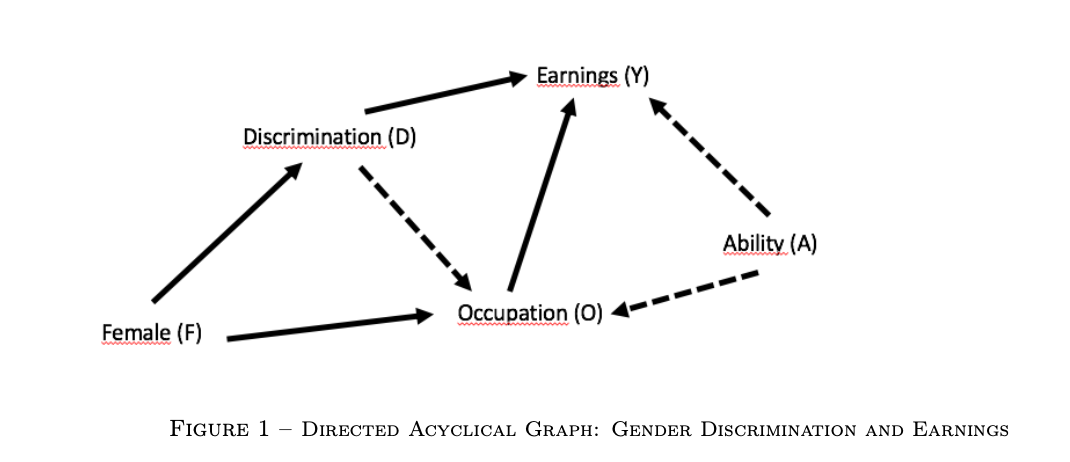
\includegraphics[width=0.5\textwidth]{Image 1.png}
    \caption{}
    \label{fig 1}
\end{figure}
\textbf{A researcher wants to estimate the effect of gender discrimination on earnings. To deconfound the causal effect, he/she develops the causal diagram shown in Figure \ref{fig 1}. All variables except A are observed in the dataset. $F$ is a dummy variable that equals unity if a person is female. $0$ is a set of dummy variables for broad occupational categories. $D$ is a dummy variable indicating if a person is being discriminated or not. Assume that only women are discriminated against. The arrow from $D$ to $O$ is dashed because it is theoretically unclear whether we should expect an effect of discrimination on occupation.}\\
\textbf{a) Provide an intuitive explanation for each arrow in Figure \ref{fig 1}. Provide an explanation for the absence of an arrow between $F$ and $Y$ . In your view, should there be additional arrows and/or variables in the diagram? If so, which ones?}\\
\textbf{b) Write out the paths from $D$ to $Y$ . Now assume that you observe ability and can control for it. Explain whether it makes sense (or not) to additionally control for the following: i) only $F$ ; ii) only $O$; iii) both.}\\
\textbf{c) Assume that $A$ is unobservable. Explain why controlling for $O$ can lead to collider bias.}\\
\textbf{d) Illustrate the collider problem in a simulation based on the above causal diagram. To do so, create a (simulated) dataset that represents all the arrows in Figure 1. It is sufficient to approximate O with one dummy variable. You will have to run several regressions; at the least, show the following regressions: i) $Y$ on $D$; ii) $Y$ on $D$ controlling for $O$; iii) $Y$ on $D$ controlling for $O$ and $A$. Run further regressions if needed and explain why the coefficients differ (or not). The task is here to show convincingly that controlling for variables on the causal path can lead to collider bias. This is what researchers would do in methodological papers, conference discussions or referee reports.}\\
\newpage
\subsection{2.2 
Application: Miscarriages and the Outcomes of Subsequent Children}
\textbf{In a new paper, the authors study the effect of a mother having a miscarriage on the outcomes of sub-sequent children. Prior research has shown that miscarriages, while common, can have traumatic effects on women and, by extension, on families. It is thus plausible that a miscarriage affects the outcomes of children that were subsequently conceived and born, for example through changes in parenting styles.
The authors undertake several steps towards establishing causality. They refer to a large number of studies showing that the likelihood of having miscarriages appear to be unrelated to mother or family characteristics, and provide balancing tests in support of this assumption. A second challenge is to find a suitable control group. They restrict the sample to families with two children; the treatment group had a miscarriage in between the births of both children, the control group had no miscarriage.}\\
\textbf{a) While this identification strategy appears plausible at first, the choice of control group may induce a bad control problem (i.e. the choice is equivalent to conditioning on a mediator). Construct a DAG to explain where the bad control problem could lie and why this might bias the estimates (Hint: it has to do with the decision to have another child after a miscarriage). Discuss under what conditions the assumption that having a miscarriage is random is sufficient for establishing causality.}\\
\textbf{b) Using potential outcomes notation, derive the bias in the estimation of the ATE that results from the bad control problem found in a). Explain in what direction the bias could likely go.}\\
\textbf{c) Propose tests that could potentially show that the bias is quantitatively unimportant (after all, no identification strategy is perfect; so showing that a bias does not matter is often what is needed). Please be brief here.}\\


\end{document}
